%%%%%%%%%%%%%%%%%%%%%%%%%%%%%%%%%%%%%%%%%%%%%%%%%%%%%%%%%%%%%%%%%%%%%%%%%%%%%%%%%
%% Document: Thesis for PhD at UC Riverside                                    %%
%% Title: Investigating the evolution of environmental and biotic interactions %%
%%          in basal fungal lineages through comparative genomics              %%
%% Author: Steven Ahrendt                                                      %%
%%%%%%%%%%%%%%%%%%%%%%%%%%%%%%%%%%%%%%%%%%%%%%%%%%%%%%%%%%%%%%%%%%%%%%%%%%%%%%%%%
%% APPENDIX FIGURES %%
%%%%%%%%%%%%%%%%%%%%%%

% Flagellar heat map from James et al 2009
\begin{figure}
  \centering
  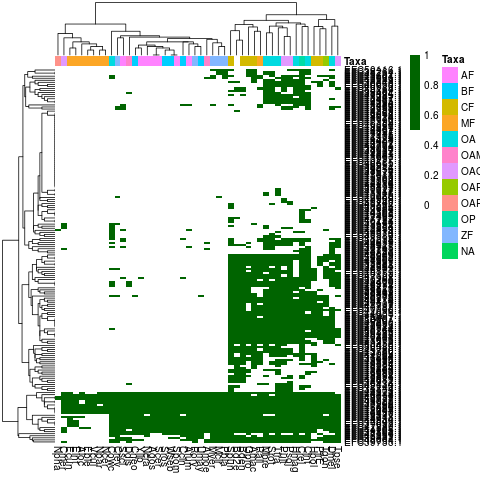
\includegraphics[width=4in]{./Appendix/img/flagDataHeatmap.png}
  \caption[Heatmap cluster analysis of flagellar proteins from \textit{Naegleria gruberi}]{Protein copies identified in proteomes of interest are normalized to indicate presence and absence only, where green indicates that one or more copies were found. Proteins are listed on the right, and proteomes given on the bottom. Both rows and columns are clustered by the "complete" method}
  \label{fig:AppFlag_heatmap}
\end{figure}
